%File: RBM.tex
%Date: Tue Dec 31 03:29:37 2013 +0800



\subsection{CRBM}

\begin{frame}{CRBM}
  \begin{reference}{4mm}{85mm}
Chen, Hsin and Murray, Alan F, 2003,
Continuous restricted Boltzmann machine with an implementable training algorithm
  \end{reference}
  \begin{itemize}
    \item \textbf{Restricted Boltzmann Machine} is a generative stochastic two-layer neural network.

    \item \textbf{Continuous RBM} extends RBM to real-valued inputs.
      \pause
    \item RBM has the ability to reconstruct a layer similar to input layer.
      The difference between the two layers can be a used to measure the fitness of an input to the model.

    \item Therefore, RBM can be a substituion to GMM.
  \end{itemize}

  \begin{center}
    \visible<2>{\includegraphics[width=0.4\textwidth]{res/rbm-original.png}}
    \visible<2>{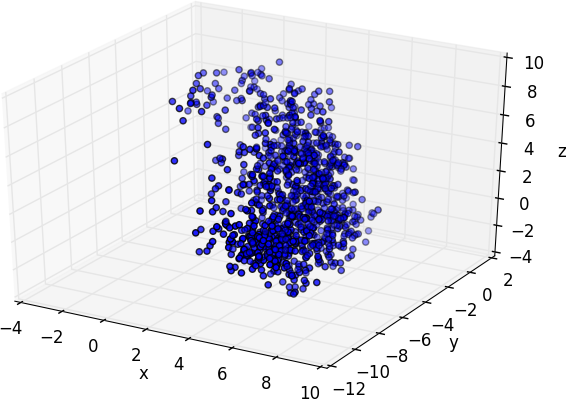
\includegraphics[width=0.4\textwidth]{res/rbm-reconstruct.png}}
  \end{center}
  \vspace{1em}
\end{frame}

\begin{frame}{RBM Results}
  Results of CRBM, tested with 5 secs
  of utterance.
  \begin{center}
    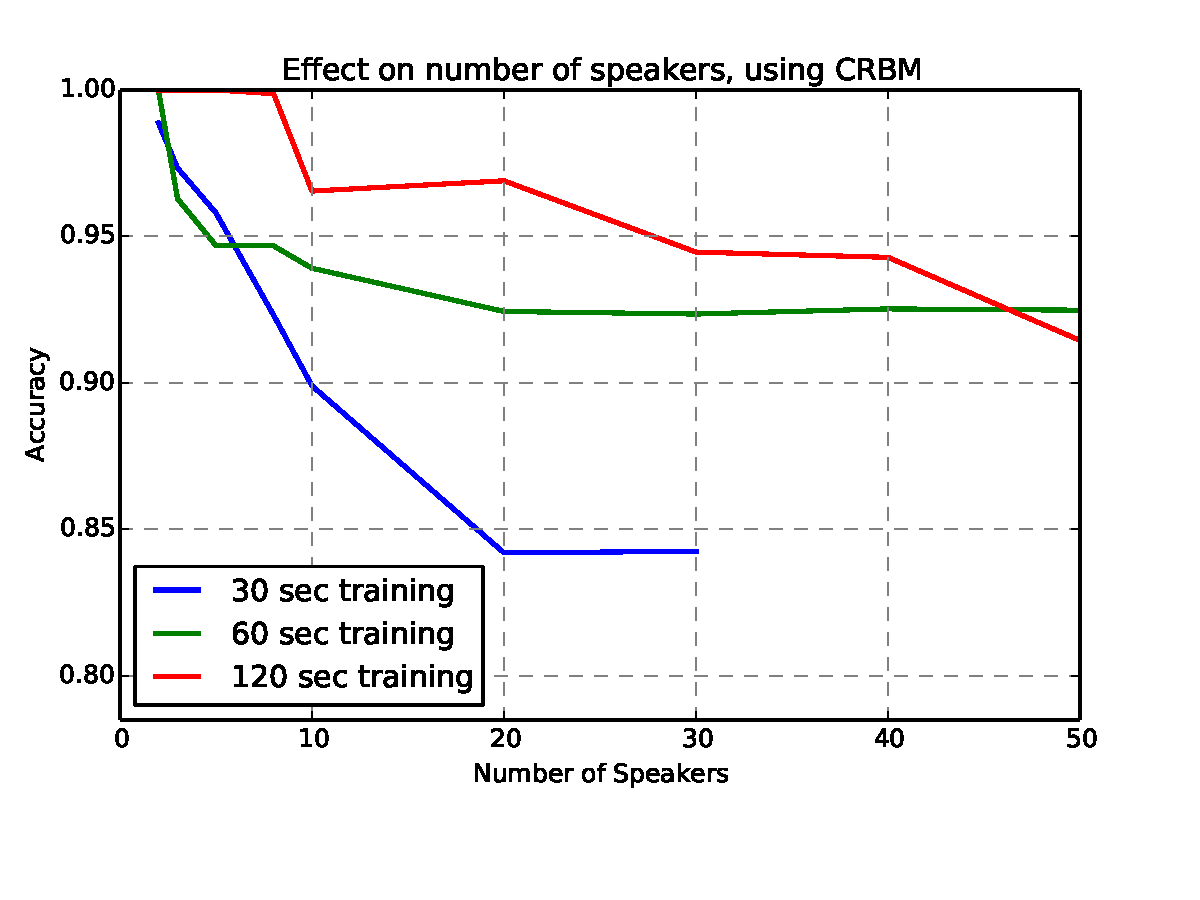
\includegraphics[width=0.7\textwidth]{res/crbm.pdf}
  \end{center}
\end{frame}

